\section{Solución propuesta}

En esta sección se presenta una breve descripción de la solución que se propone, el principal objetivo de esta sección es poder explicar qué estructuras utilizaron, cuál es el flujo de su programa, explicación sobre las líneas/secciones más importantes del código, dificultades que encontraron, etc.
—
Las reservas de habitaciones pueden ser un problema, dado que hay que tener en cuenta las fechas disponibles y la coordinación entre el cliente y la posada. Por eso, lo que nosotros proponemos es una aplicación web que provea a los clientes una forma sencilla de reservar, sin pasar por consultas por mail o Whatsapp. En vez de ello, el interesado busca en un calendario las fechas en las que le gustaría hospedarse y la página le realiza la consulta. Acto seguido, el cliente confirma la reserva.

La estructura del proyecto consta de una API (Application Program Interface) y de un servidor web, ambas son aplicaciones separadas que actúan de la siguiente forma:

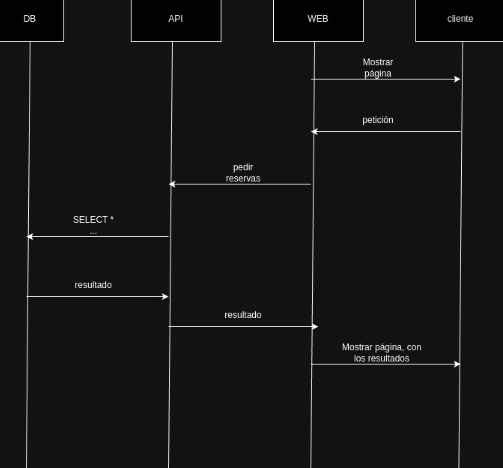
\includegraphics{estructura}
